\documentclass[12pt,a4paper]{article}

\usepackage[utf8]{inputenc}
\usepackage[T1]{fontenc}
\usepackage{times}
\usepackage[margin=2.5cm]{geometry}
\usepackage{setspace}
\doublespacing
\usepackage[british]{babel}
\usepackage{csquotes}

\usepackage{graphicx}
\graphicspath{{../figures/}}
\usepackage{float}
\usepackage{placeins}
\usepackage{amsmath,amssymb}
\usepackage{booktabs}
\usepackage{makecell}
\usepackage{enumitem}
\usepackage[colorlinks=true,linkcolor=blue,citecolor=blue,urlcolor=blue]{hyperref}
\usepackage[style=apa,backend=biber,natbib=true]{biblatex}
\addbibresource{references.bib}
\usepackage{lineno}
\linenumbers

\begin{document}

\begin{center}
{\LARGE\bfseries Stagnation before exit: performance progression and retention in youth track and field\par}
\vspace{0.6em}
{\normalsize Anonymised manuscript\par}
\end{center}

\section*{Abstract}

\noindent Declining competition volume foreshadows exit from organised youth sport; whether the athlete's own performance development adds information is untested in population data. Mastery-experience accounts of motivation predict that visible personal progress retains athletes, most strongly where rank-based competence is scarce, as for athletes born late in the selection year. Using the Norwegian Athletics Federation's registry, we followed athletes born 1998--2005 with scorable age-graded points in their main event group at ages 13--14 and 15--16 (n = 3\,877; 53\,\% female), of whom 654 (16.9\,\%) were later active as seniors (age $\geq$20). Progression was the change in age-graded points (mean of three best scores) between the two windows. In logistic regression adjusted for sex, cohort, performance level, competition volume and the number of scored results, progression predicted senior activity (odds ratio [OR] 2.24 per SD, 95\,\% CI 1.90--2.63) and modestly improved discrimination (cross-validated AUC 0.854 to 0.866). The association replicated across birth cohorts and held at equal numbers of results, with event-equated points, and among athletes still competing after age 16 (OR 1.83). Aligned at exit, dropouts held their performance level until the final season and fell about 12 points below it as their competition volume collapsed. The pre-specified progression $\times$ birth-quarter interaction was null (OR 0.95, 95\,\% CI 0.84--1.06), and evidence for a mediated pathway was weak. Low progression accompanies and precedes exit, beyond volume and level, but the relative-age-specific form of the mastery prediction was not supported. Current form, not early rank, is what the retention signal tracks.

\vspace{0.5em}
\noindent\textbf{Keywords:} youth sport; dropout; athlete retention; performance development; mastery experience; relative age; track and field

\newpage

\section{Introduction}

Withdrawal from organised youth sport is extensive, and its documented predictors are mostly motivational and structural rather than performance-related. Loss of enjoyment is the most consistently reported reason for leaving \citep{crane2015} and the main prospective predictor \citep{vanyperen2021}; costs and social background shape the reasons young people give for leaving \citep{espedalen2022}; a large share of turnover in talent systems is the system's own de-selection \citep{gullichbarth2026}, and much of the attrition at the youth-to-senior transition is structural rather than individual \citep{filo2026}; and markers of early specialisation have failed to predict actual dropout when tested directly \citep{larson2019}. Performance itself has an ambiguous role. Junior performance predicts senior performance poorly \citep{kearney2018,barth2022,gullich2025}, and in the most direct registry test to date, performance level at a single early milestone discriminated senior retention somewhat less well than a simple behavioural signal, how often the athlete competed, though it added complementary information \citep{guttormsen2026dropout}.

\subsection{Mastery experience as a retention mechanism}

There is, however, a theoretical reason to expect performance to matter for retention in a particular form: not as rank, but as the athlete's own visible progress. In the self-efficacy theory of \citet{bandura1977}, performance accomplishments, the enactive mastery experiences, are the most influential of the four sources of efficacy expectations: successes raise them and repeated failures lower them, and efficacy expectations in turn determine how much effort is expended and how long it is sustained. Seeing oneself improve at a task is therefore the most direct route to persisting at it. Perceived competence occupies the same position in self-determination theory, as one of the basic psychological needs whose satisfaction supports intrinsic motivation and persistence \citep{ryan2000}, and in the developmental model of effectance motivation of \citet{harter1978}, in which successful mastery attempts generate the positive affect that motivates further attempts. Achievement goal theory adds the distinction that makes the prediction testable with performance records. Under a self-referenced (task) conception of ability, improvement over one's own previous performance signals competence; under an other-referenced (ego) conception, competence is signalled by outperforming others \citep{nicholls1984}. A task-involved athlete can therefore experience competence while ranked low, provided they are improving. These accounts converge on one prediction: athletes stay where they can observe their own progress. Retrospective comparisons of dropouts with engaged athletes point in a related direction: dropouts had been the youngest in their training groups and had reached developmental milestones earlier \citep{fraserthomas2008}, and perceptions of competence recur among the factors associated with dropout across studies \citep{crane2015}.

Track and field is an unusually clean setting for this prediction. Every result is an objective, repeatable measure of the athlete's own performance, and in Norway age-graded points printed on youth result lists and used for club awards translate those marks into a common scale. Visible personal progress is therefore not a researcher's abstraction but a signal athletes actually receive. The prediction also has a specific corollary. Competence can be fed from two sources, self-referenced progress and other-referenced rank, and relatively younger athletes in a calendar-year class, who are on average less mature than their classmates, have less access to the second. If mastery experience retains athletes, it should do so most where rank cannot: the progression--retention association should be stronger among athletes born late in the selection year. A population-wide analysis of relative age in this registry, which found the birth-quarter skew fully established at age 10 and stable to age 25, proposed exactly this interpretation and stated the test: whether within-athlete performance \emph{progression}, rather than performance level, predicts retention among relatively younger athletes specifically \citep{guttormsen2026rae}.

\subsection{The gap}

Two further analyses of the same national registry frame the gap. A longitudinal study of performance development showed that a third to more than half of a cross-sectional youth top list is replaced from one year to the next, so that the best performers at one age are largely different people from the best at the next, and that the apparent late-teen plateau in such lists is an artefact of this compositional turnover; it did not study who exits or why \citep{guttormsen2026development}. A 14-year cohort study showed that exit is behaviourally foreshadowed: future dropouts' competition volume fell 12\,\% below their own earlier level two seasons before exit and 23\,\% one season before, and volume at ages 13--14 predicted senior retention better than age-graded performance level did \citep{guttormsen2026dropout}. To our knowledge, no study with complete national coverage has linked objective within-athlete performance trajectories to a prospectively defined exit outcome while adjusting for the behavioural participation signal.

\subsection{The present study}

This study performs that test. Among athletes still competing at ages 15--16, we ask three pre-specified questions. \textbf{H1:} does within-athlete progression from ages 13--14 to 15--16 predict being active as a senior, beyond sex, performance level, competition volume (level and change), and the number of results the progression measure is computed from? \textbf{H2:} is the association stronger among relatively younger athletes, as the reinforcement corollary of the mastery account predicts? \textbf{H3:} does progression, rather than level, carry the performance-related signal? Interpretation rules were fixed in advance. In particular, a null or weak H1 would \emph{not} falsify the mastery account, because the registry cannot distinguish disengagement from transfer to another sport in which the athlete is also progressing. The plan framed H2 as the mastery-specific test, so a positive H1 with a null H2 is consistent with a general progression--retention link without supporting the relative-age-specific mechanism. The analysis plan, including hypotheses, estimands, model specifications, and these interpretation rules, was written and committed to version control before any exposure--outcome model was estimated; the study was not preregistered on an external registry.

% ════════════════════════════════════════════════════════════

\section{Methods}

\subsection{Data source and design}

The Norwegian Athletics Federation's results database records every sanctioned competition result in Norway, plus Norwegian athletes' results abroad, and holds results electronically from 2011; coverage in 2011, the first electronic season and the oldest cohort's age-13 season, is thinner than later, which the cohort terms absorb. We used a frozen extract of 29 October 2026 (results dated on or before that day). Before analysis we removed 12\,990 board-jump results that re-imports in 2026 had copied from an identical take-off-zone result (same athlete, date, mark and wind; almost all at age 13, and listed in the source only under the zone event), 5\,780 such copies from multi-day meets, dated to the meet's first day while the zone result lies one to six days later, and 746 exact duplicates, mostly meets stored twice. These corrections, and the scoring of every event specification for which the tables give a norm (some had initially been left unscored), were made after the first estimation; they enlarged the primary sample from 3\,808 to 3\,877 athletes and raised the H1 odds ratio from 2.02 to 2.24. The design is a retrospective landmark cohort reported according to STROBE \citep{vonelm2007}. Age is calendar-year age (competition year minus birth year), the basis of age classes in Norwegian athletics.

\subsection{Sample}

All athletes born 1998--2006 entered the extraction (n = 32\,447); 12\,938 had at least one approved result at age 13--14. The landmark condition --- at least one approved result at ages 13--14 \emph{and} at 15--16 --- was met by 4\,910 athletes, of whom 4\,909 had known sex, 4\,475 of them born 1998--2005. Prediction is made from the end of the age-16 season, so the conditioning on early-adolescent survival is explicit rather than hidden \citep{anderson1983}. Among these, we excluded 578 athletes without scorable age-graded results in their main event group in both windows (among them athletes who left their original event group entirely; a sensitivity analysis recovers some of them) and 20 athletes in sex $\times$ event-group cells with fewer than 20 athletes. The primary sample comprises 3\,877 athletes born 1998--2005, all with at least nine years of follow-up; the 434 athletes born 2006 were retained only for a secondary outcome. Of the primary sample, 654 (16.9\,\%) met the senior-activity outcome. Within the primary sample, 27 athletes lacked an exact birth date and were excluded from the birth-quarter analyses only (n = 3\,850); in the wider landmark sample the corresponding number is 43. The full sample flow, including the H2 and exit-aligned subsamples, is given in the Supplementary material (Table S1), and a completed STROBE checklist accompanies the submission.

\subsection{Exposure: within-athlete progression}

Each result at ages 13--16 (and at 17--19 for the descriptive trajectories) was converted to age-graded points with the Norwegian federation's Tyrving tables, which score a performance against age-, sex-, and event-specific reference standards; we used a workbook-exact implementation validated cell-by-cell against the official tables in earlier work on this registry \citep{guttormsen2026dropout,nfif2014}, with every event specification for which the tables give a norm scored. Because the tables are age-calibrated, a constant score in one event means developing exactly as the age norms expect; a falling score means falling behind them. The tables are not equally demanding across events, however, so a change of event within the main group also moves the score; an event-equated sensitivity analysis removes each event's offset, estimated within athlete-seasons (boys' throwing implements change at age 16, so these offsets are identified only within the two sets of implements, each of which keeps its mean score).

The athlete's \emph{main event group} is the event category with most results at ages 13--14 (in the primary sample sprints, jumps, middle distance or throws; the few athletes whose modal category was another, such as hurdles or race walking, were removed by the scorability and cell-size rules). Progression $\Delta$ is the mean of the three best scores in the main event group at ages 15--16 minus the same quantity at 13--14 (the mean of all scored results where a window has fewer than three, which applies to 1\,250 athletes in at least one window). We used the mean of the three best rather than the single best because a maximum rises mechanically with the number of attempts, which would entangle progression with competition volume. The mean of the three best still rises with the number of scored results, so the number in each window ($k_{13}$, $k_{15}$) enters all models as covariates, and a sensitivity analysis compares the windows at equal numbers of results (the expected mean of the three best over all subsets of the smaller of the two counts from each window, computed exactly). Manual-timed results were excluded from scoring; indoor and outdoor marks were pooled, with an outdoor-only sensitivity analysis. Progression and level were standardised within sex $\times$ main event group over the primary sample, since the tables are unequally demanding across event groups; volumes were standardised to the primary-sample SD. For interpretation, one SD corresponds to approximately 114 age-graded points for progression (range 74--154 across sex $\times$ event-group cells), 178 points for baseline level, and 16 and 17 competition days for the two volume windows. Throughout, ``dropout'' denotes disengagement from sanctioned competition; some leavers may continue training or unsanctioned activity.

\subsection{Outcome}

The primary outcome, identical to the earlier cohort study of this registry \citep{guttormsen2026dropout}, is \emph{active senior}: at least two approved results in the same calendar year at age 20 or older, with follow-up to the extract date. Secondary outcomes were at least one result at age $\geq$20; at least one result at age $\geq$18 (allowing the 2006 cohort); and at least two results in a year at ages 20--21 (a fixed window equalising opportunity across cohorts).

\subsection{Covariates}

Sex; birth cohort; performance level (mean of three best scores at 13--14, standardised); competition volume as distinct competition days at 13--14 and at 15--16, so that volume enters as level \emph{and} change, mirroring the earlier cohort study; $k_{13}$ and $k_{15}$; and baseline club (modal club at 13--14) with a club-size proxy (log of the number of study athletes in the club). Region could not be adjusted for: the registry records the competition district for under 1\,\% of meets. Birth quarter (Q1--Q4) was computed from exact birth dates.

\subsection{Statistical analysis}

Nested logistic models were fitted on the primary sample: M0 (sex, cohort, club size), M1 (M0 + level + volume 13--14 + volume 15--16 + $k_{13}$ + $k_{15}$), and M2 (M1 + $\Delta$). H1 is the OR per SD of $\Delta$ in M2 and the gain in discrimination from M1 to M2, estimated by stratified 5-fold cross-validation repeated 20 times, with calibration slope and Brier score from out-of-fold predictions. Percentile intervals over the 20 repetitions describe only the Monte Carlo variability of the resampling procedure on this one dataset; sampling uncertainty for AUC differences is therefore quantified with paired DeLong 95\,\% confidence intervals computed on the out-of-fold predictions, and the two kinds of interval are labelled as such wherever both appear. One property of M2 should be stated openly: because $\Delta$ is the difference between the 15--16 and 13--14 scores, a model containing both baseline level and $\Delta$ is a reparametrisation of one containing the 13--14 and 15--16 levels. The progression estimand is therefore equivalent to asking how much the \emph{later} performance level adds given the earlier one --- deliberately the same ``level and change'' logic that \citet{guttormsen2026dropout} applied to competition volume. H2 adds a $\Delta \times$ birth-quarter linear interaction (Q1$\to$Q4), with stratified ORs for athletes born Q1--Q2 and Q3--Q4. H3 compares cross-validated AUC between (sex + volumes + $k$ + $\Delta$) and (sex + volumes + $k$ + level). Secondary analyses were a landmark Cox model among athletes still competing after age 16 (time from the end of the age-16 season; censoring athletes active in 2025--2026) and exit-aligned descriptive trajectories: among non-censored dropouts whose final season fell at ages 16--19, the within-athlete change in points and in competition days in each of the last three active seasons (the final season and the two before it), relative to the athlete's own level three seasons before exit (bootstrap CIs for medians). Because the mean of the three best rises with the number of results and dropouts compete less towards the end, each season's points were compared with the reference season at equal numbers of results (the expected value over all subsets of the smaller of the two counts, computed exactly); the season median, which does not depend on the count, is reported alongside.

Pre-specified robustness analyses varied the exposure (season best; mean of all results; wind-legal marks only; progression in the best event group at 15--16, recovering event-group switchers), required $k \geq 2$ in both windows, excluded cohorts whose 15--16 window overlapped the COVID-19 seasons 2020--2021 (born 2004--2005) and tested a COVID-window interaction, varied the outcome, replicated the estimate in the two cohort halves (born 1998--2001 and 2002--2005), and re-estimated under club-clustered robust standard errors and GEE with exchangeable club correlation. A specification check regressed the outcome on progression \emph{within} the baseline window (age 13 to 14). After estimation, regression to the mean was also examined directly by entering both period levels instead of level and change: under a pure baseline-measurement artefact the earlier level would carry a positive coefficient given the later one. Added after estimation were the analyses at equal numbers of results, event-equated and outdoor-only points, spline terms for result counts and volumes, at least three scored results per window and restriction to athletes still competing after age 16, as were the mediation analysis, the progression quintiles, the level tertiles, the progression $\times$ level and progression $\times$ sex interactions, and the inclusive switcher sample. E-values quantified the unmeasured confounding needed to explain the primary association away \citep{vanderweele2017}; because the outcome is common (16.9\,\%), the odds ratio was converted to a risk ratio by the square-root approximation recommended for common outcomes, and the E-value statement is on the risk-ratio scale. Analyses used Python 3.13.7 with pandas 2.3.3, numpy 2.4.1, statsmodels 0.14.6, scikit-learn 1.8.0 and lifelines 0.30.3. Two-sided $\alpha$ = 0.05 for H1; H2 was directional in its prediction (the sign of the interaction) but is tested and reported with conventional two-sided intervals. The opportunity-unequal primary outcome definition keeps all available follow-up and maximises events; the fixed-window outcome at ages 20--21 equalises opportunity across cohorts and is reported in robustness, and the partially observed 2026 season contributes results through 29 October. Deviations from the analysis plan are listed in the Supplementary material (Section S3).

\subsection{Sample size and precision}

The sample is the complete national population meeting the landmark condition, so no sampling decision was open to a power calculation. The size of the primary sample and the number of senior retainers were, however, known and recorded in the analysis plan before any exposure--outcome model was estimated (3\,808 athletes and 648 events at the plan stage; 3\,877 and 654 after the data corrections described above), and the effect size anchoring the design was the odds ratio of 2.04 per SD for baseline competition volume reported for the same outcome in the same registry \citep{guttormsen2026dropout}. By the method of \citet{hsieh1998} for a standardised continuous predictor in logistic regression, with an event probability of 0.17 and allowing for a squared multiple correlation of 0.25 between progression and the covariates, the plan-stage sample gave 80\,\% power at two-sided $\alpha$ = 0.05 to detect an odds ratio of about 1.15 per SD, and 90\,\% power for about 1.18, both far below the benchmark. For the H2 interaction, assuming progression and birth quarter to be uncorrelated and taking the observed SD of birth quarter (1.09), the same sample gave 80\,\% power for an interaction odds ratio of about 1.14 per quarter. Precision is reported throughout as 95\,\% confidence intervals.

\subsection{Ethics and transparency}

The data are public competition results. In line with the Norwegian children's sport regulations, no performance analysis involves ages below 13. No individual athlete is identified, and dropout is never characterised at the individual level. As for the earlier studies of the same registry, the study is not medical or health research as defined by Norway's Health Research Act (Helseforskningsloven \S\S~2 and 4), so approval by a Regional Committee for Medical and Health Research Ethics was not required, and Sikt (the Norwegian Agency for Shared Services in Education and Research) confirmed that the use of the data raises no data-protection concerns [Sikt reference number and date to be inserted at submission]. Analysis code and aggregate outputs are version-controlled; athlete-level files are kept outside the repository and are regenerable from the registry.

% ════════════════════════════════════════════════════════════
\section{Results}

\subsection{Sample and descriptive differences}

Table~\ref{tab:char} describes the primary sample. Future senior retainers differed from future dropouts already at ages 13--14: they competed more than twice as often (median 29 vs.\ 12 competition days) and scored higher (median 938 vs.\ 810 age-graded points), and over the following two seasons their median progression was +37 points against $-$12 for dropouts. Part of that contrast is mechanical: dropouts had far fewer scored results at 15--16 (median 5 against 30), and the mean of the three best rises with the number of results. Compared at equal numbers of results, dropouts' median progression was +7 points against +35 for retainers, and 45.8\,\% of dropouts against 24.3\,\% of retainers had negative progression (56.5 and 28.1\,\% without equalising; Table~\ref{tab:char}). Figure~\ref{fig:age} shows the season-by-season picture, with the same result-count caveat: among athletes competing in their main event group at a given age, future retainers pulled away from the age norms (median 900 points at 13, 975 at 16), while future dropouts started about 110 points lower (median 789 at 13) and tracked roughly parallel to the norms, with an apparent late rise (822 at 16, 851 at 18) that reflects progressive selection, since ever fewer and increasingly persistent dropouts remain in the group at higher ages.

\begin{table}[H]
\centering
\caption{Characteristics of the primary landmark sample (born 1998--2005), by senior-retention status.}
\label{tab:char}
\small
\resizebox{\textwidth}{!}{\begin{tabular}{lccc}
\toprule
Characteristic & All & Senior retainers & Future dropouts \\
\midrule
n & 3\,856 & 652 & 3\,204 \\
Female, \% & 53.2 & 46.6 & 54.6 \\
Cohort A (born 1998--2001), \% & 47.8 & 49.5 & 47.5 \\
Main event group: sprints, \% & 37.5 & 36.2 & 37.7 \\
Main event group: jumps, \% & 28.0 & 25.8 & 28.4 \\
Main event group: middle distance, \% & 19.5 & 19.9 & 19.4 \\
Main event group: throws, \% & 15.1 & 18.1 & 14.5 \\
Born Q1, \% of those with a birth date & 29.6 & 29.9 & 29.6 \\
Born Q4, \% of those with a birth date & 18.6 & 17.2 & 18.8 \\
Competition days 13--14, median (IQR) & 15 (5--28) & 29 (15--43) & 12 (4--24) \\
Competition days 15--16, median (IQR) & 10 (3--25) & 34 (22--48) & 7 (2--18) \\
Scored results 13--14 ($k_{13}$), median (IQR) & 14 (5--27) & 27 (14--45) & 12 (4--23) \\
Scored results 15--16 ($k_{15}$), median (IQR) & 8 (2--21) & 30 (16--47) & 5 (2--15) \\
Age-graded points 13--14, median (IQR) & 832 (710--925) & 940 (845--1010) & 812 (691--902) \\
Age-graded points 15--16, median (IQR) & 828 (702--933) & 985 (900--1043) & 798 (677--896) \\
Progression, points, median (IQR) & $-$4 ($-$60--53) & 36 ($-$4--82) & $-$14 ($-$71--43) \\
\bottomrule
\end{tabular}
}
\vspace{0.3em}
\parbox{0.92\textwidth}{\footnotesize Exact birth dates exist for 3\,850 of the 3\,877 (99.3\,\%); among these, the full quarter distribution is Q1 29.6, Q2 27.2, Q3 24.5, Q4 18.6\,\%. Equal numbers of results: both windows reduced to the smaller of the two result counts (expected value over all subsets of that size). Abbreviations: IQR, interquartile range; Q1--Q4, first to fourth quarter of the birth year.}
\end{table}

\begin{figure}[H]
\centering
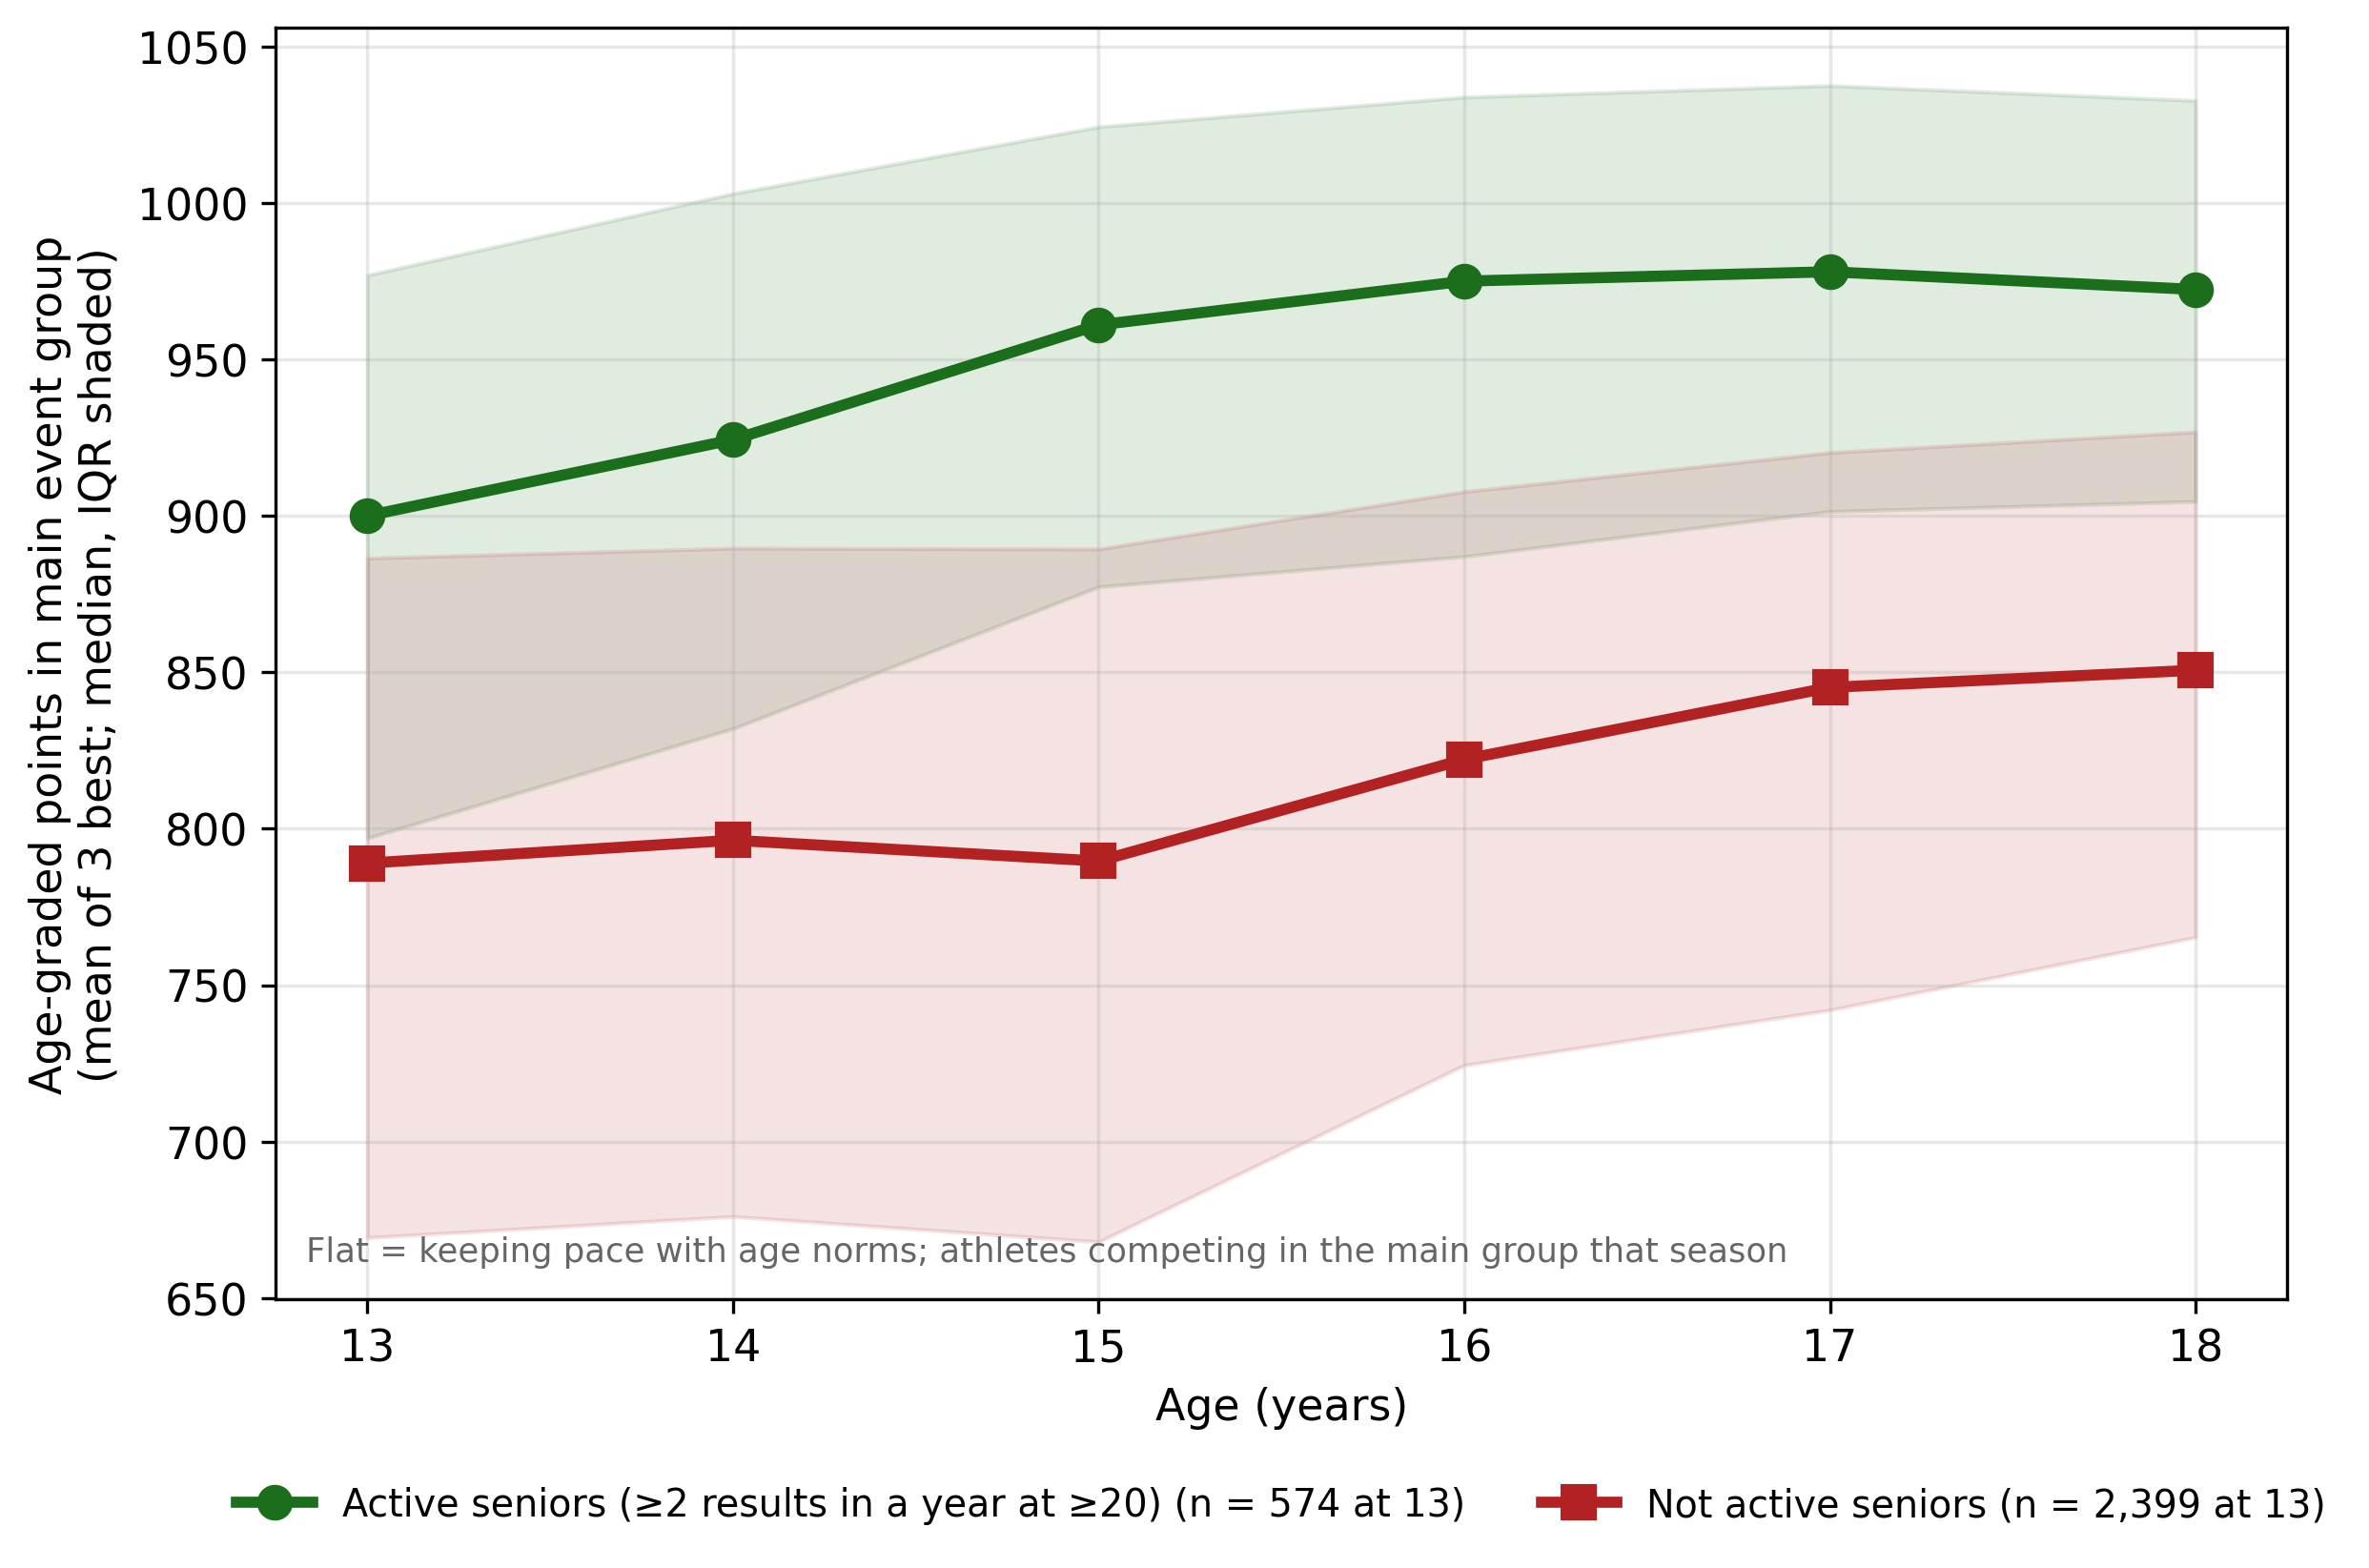
\includegraphics[width=0.95\textwidth]{fig1_performance_by_age.png}
\caption{Age-graded performance (mean of three best results in the main event group; median, IQR shaded) by age and senior-retention status, among athletes competing in the main group that season. Because the points are age-calibrated, a flat line means developing as the age norms expect. The late rise in the dropout group reflects progressive selection of the most persistent dropouts, not improvement of the group that started: the dropout curve rests on 2\,399 athletes at 13, 3\,060 at 15, 1\,034 at 17 and 571 at 18, while the retainer curve spans 574--645 at 13--14 and 508 at 18. Seasons with few results score lower on the mean of three best, which depresses the dropout curve somewhat. Abbreviation: IQR, interquartile range.}
\label{fig:age}
\end{figure}

\subsection{Progression predicts senior retention (H1)}

Table~\ref{tab:models} reports the nested models. Adding progression to the full baseline model gave OR = 2.24 per SD (95\,\% CI 1.90--2.63; $p < .001$). In the same model, competition volume at 15--16 remained the strongest predictor (OR 3.19 per SD, 95\,\% CI 2.50--4.06), volume at 13--14 added little given later volume (OR 0.82), and women were less likely to remain than men with the same level, volume, and progression (OR 0.57, 95\,\% CI 0.46--0.70; a conditional association, revisited in \S\ref{sec:sex} --- as are all covariate coefficients in these mutually adjusted models). The coefficient on baseline level rose from 1.73 in M1 to 2.56 in M2, as the reparametrisation in Methods implies: once the change is held fixed, the baseline coefficient absorbs the full weight of the implied later level. Cross-validated discrimination rose from AUC 0.854 (M1) to 0.866 (M2), a gain of 0.012 (paired DeLong 95\,\% CI 0.005--0.018, p $<$ 0.001; spread across CV repetitions 0.011--0.013), with good calibration (slope 0.96; Brier 0.097). The association was monotone across the exposure range: relative to the lowest progression quintile, the adjusted ORs for quintiles 2--5 were 1.40, 2.01, 2.94 and 5.58. The association is thus strong while the incremental discrimination beyond an already rich behavioural model is modest.

Figure~\ref{fig:quintile} shows the gradient descriptively. Within the highest tertile of later competition volume ($\geq$19 competition days over ages 15--16), senior retention rose from 21.0\,\% in the lowest progression quintile to 48.8\,\% in the highest; within the middle tertile from 4.9\,\% to 14.3\,\%. In the lowest-volume tertile ($\leq$5 days) retention was 1.0--3.6\,\% in every quintile: where engagement had already collapsed, progression distinguished little. This volume dependence was not a pre-specified hypothesis and should be read as exploratory.

Two further heterogeneity analyses ground claims made below. Across baseline-level tertiles, progression predicted retention at every level --- OR 1.79 (1.29--2.48) in the lowest, 2.23 (1.65--3.01) in the middle and 2.65 (2.01--3.51) in the highest tertile, with a non-significant progression $\times$ level interaction (OR 1.08, 0.96--1.21). The upward drift in the point estimates is consistent with measurement reliability rather than moderation: in the lowest tertile the median athlete had only three scored results at 15--16, so progression is noisier there, and among athletes with at least three scored results in both windows the tertile ORs were 2.67, 2.29 and 2.75 (interaction 1.01, 0.84--1.20). By sex, one interaction model gave a similar association in women and men --- OR 2.21 (1.77--2.77) and 2.25 (1.86--2.73), interaction p = 0.89 --- so the signal is not carried by one sex.

\begin{table}[H]
\centering
\caption{Nested logistic models for senior activity (age $\geq$20) in the primary sample (n = 3\,877; 654 events). OR (95\,\% CI) per SD unless noted.}
\label{tab:models}
\small
\begin{tabular}{lcc}
\toprule
Predictor & M1 & M2 \\
\midrule
Progression 13--14 $\to$ 15--16, per SD & --- & 2.24 (1.90--2.63) \\
Performance level 13--14, per SD & 1.73 (1.48--2.02) & 2.56 (2.13--3.07) \\
Competition days 13--14, per SD & 0.72 (0.53--0.98) & 0.82 (0.60--1.12) \\
Competition days 15--16, per SD & 3.78 (3.00--4.78) & 3.19 (2.50--4.06) \\
Scored results 13--14, per result & 1.00 (0.99--1.02) & 1.01 (0.99--1.02) \\
Scored results 15--16, per result & 1.00 (0.99--1.01) & 0.99 (0.97--1.00) \\
Female (vs.\ male) & 0.62 (0.50--0.76) & 0.57 (0.46--0.70) \\
\midrule
Cross-validated AUC & 0.854 & 0.866 \\
$\Delta$AUC M2 $-$ M1, DeLong 95\,\% CI & \multicolumn{2}{c}{0.012 (0.005--0.018); repetition spread 0.011--0.013} \\
Calibration slope / Brier (M2) & \multicolumn{2}{c}{0.96 / 0.097} \\
\bottomrule
\end{tabular}

\vspace{0.3em}
\parbox{0.92\textwidth}{\footnotesize Both models additionally adjust for birth cohort and club size. Because progression is the difference between the 15--16 and 13--14 scores, M2 is a reparametrisation of a model with both period levels; the progression OR equals the contribution of the later level given the earlier one. Abbreviations: AUC, area under the receiver operating characteristic curve; CI, confidence interval; OR, odds ratio; SD, standard deviation.}
\end{table}

\begin{figure}[H]
\centering
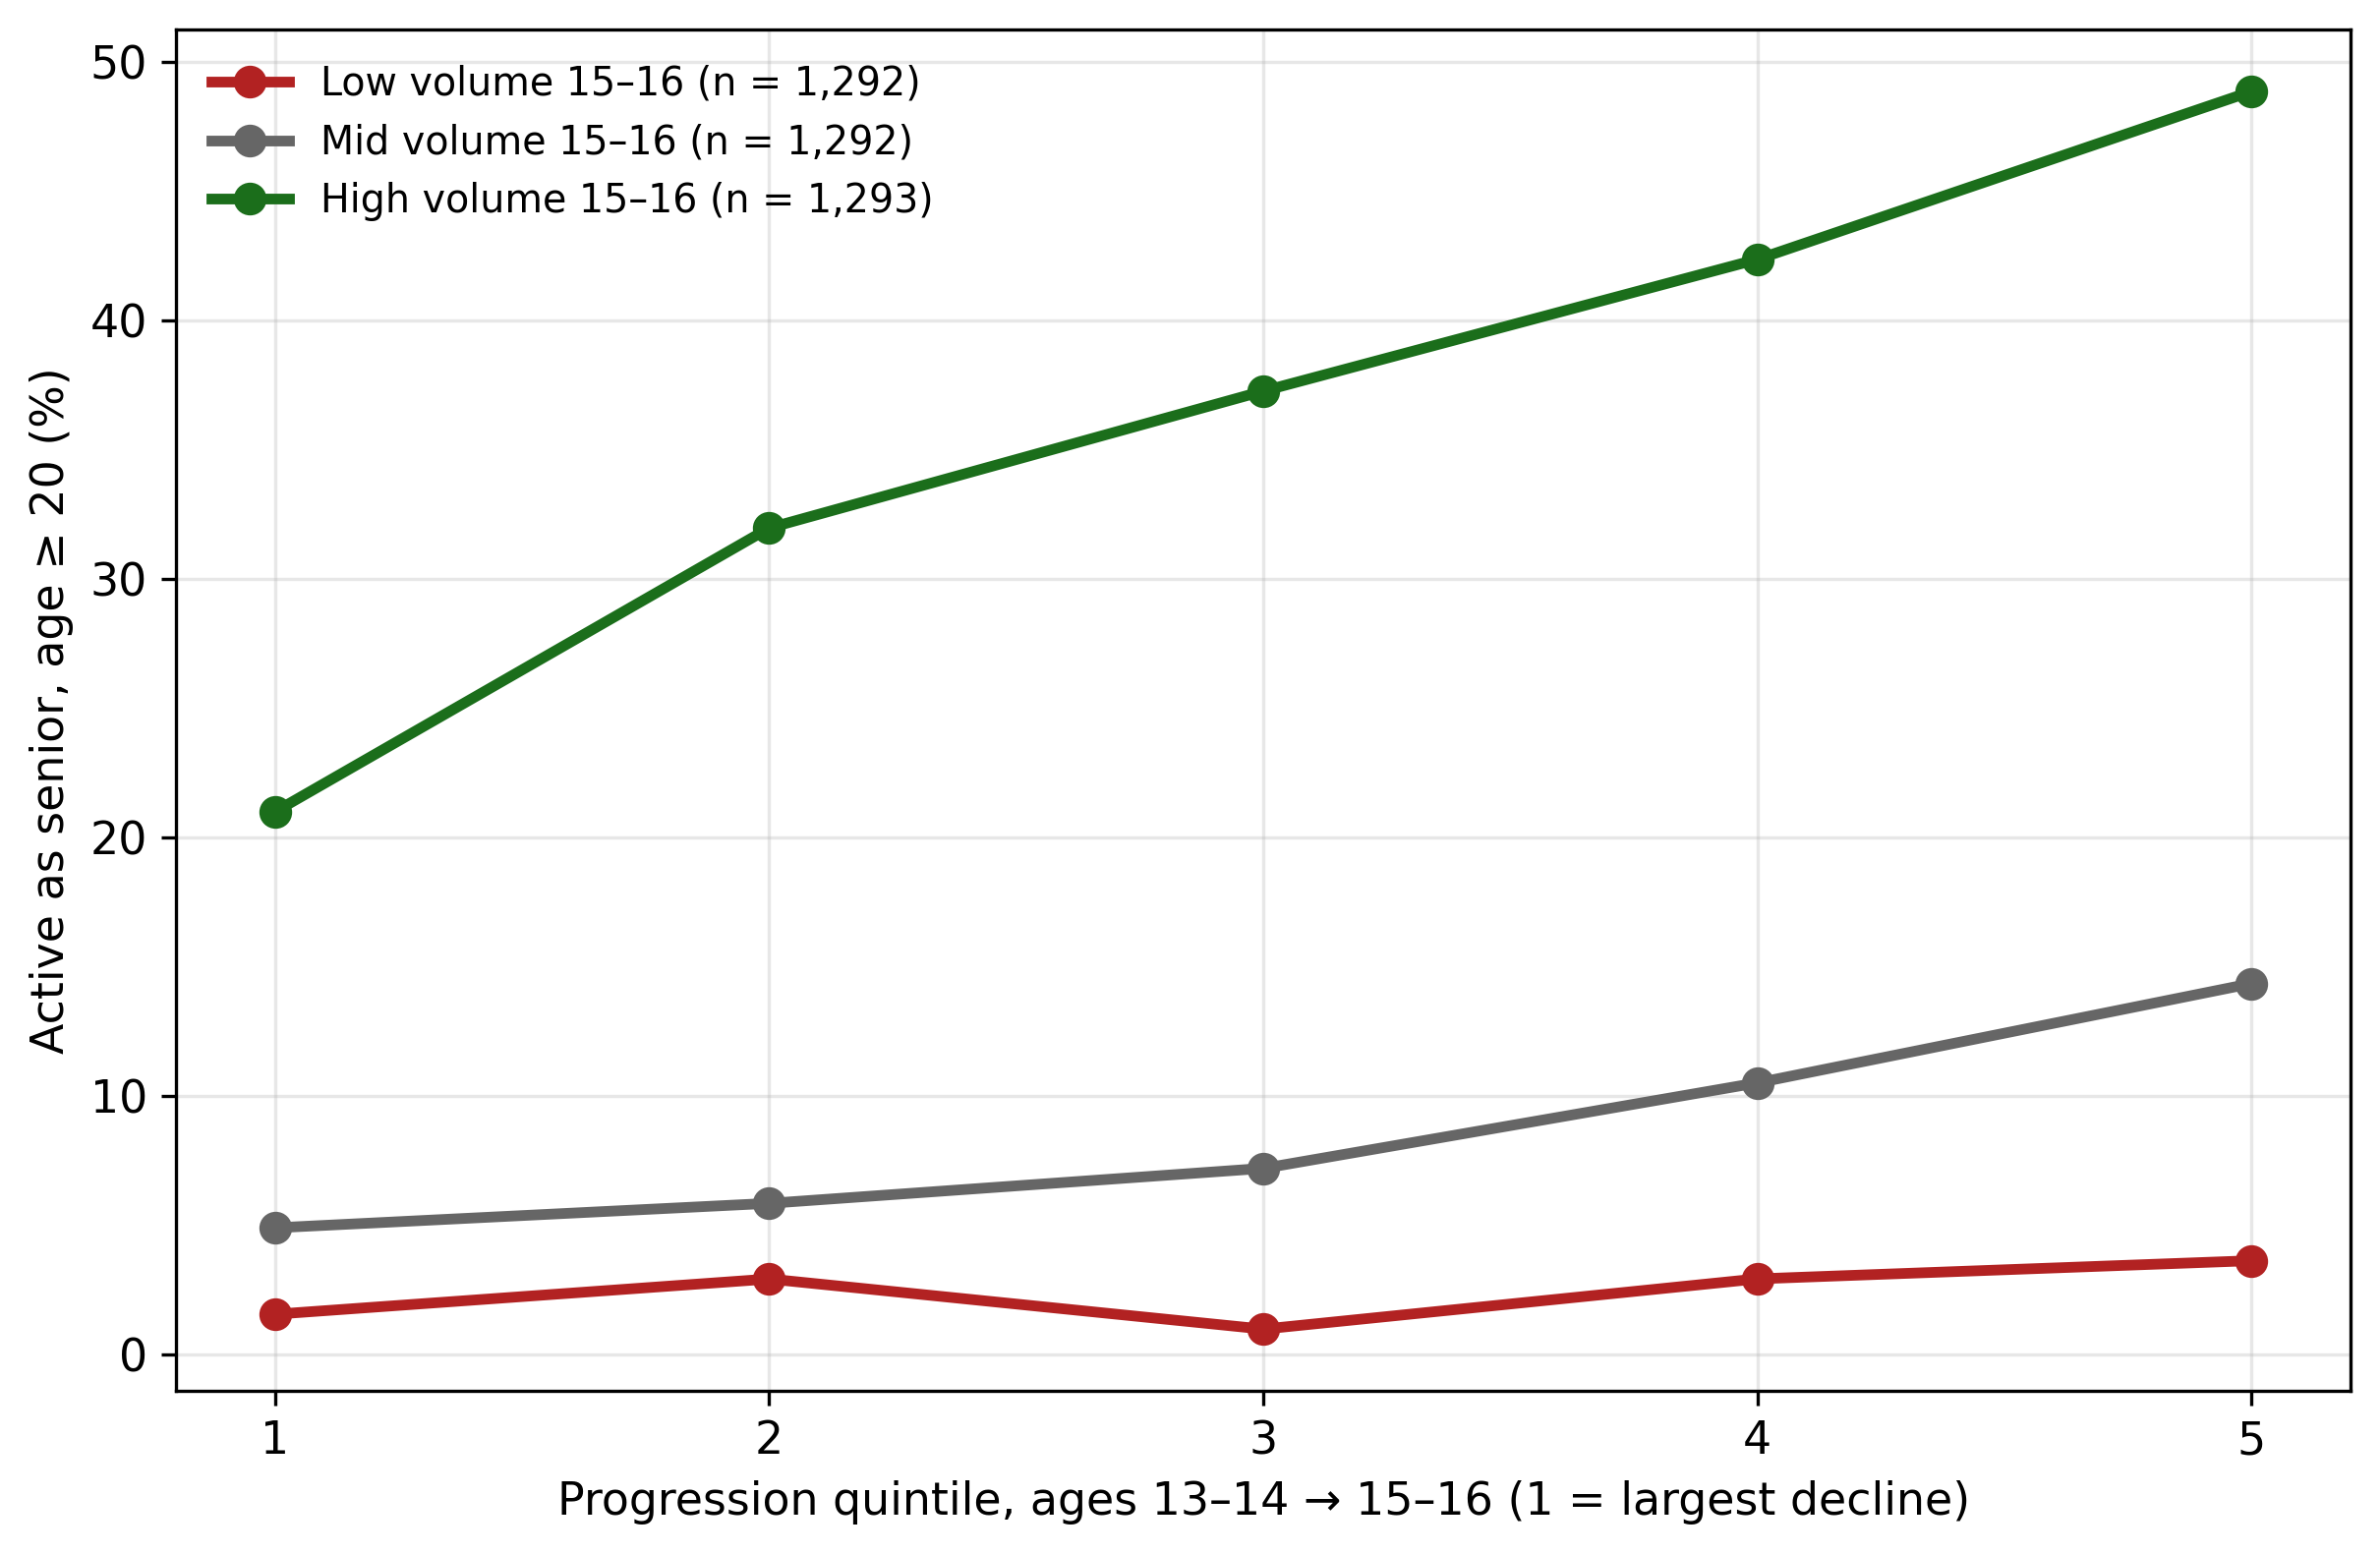
\includegraphics[width=0.85\textwidth]{fig2_retention_by_progression.png}
\caption{Senior retention by progression quintile within tertiles of competition volume at ages 15--16 (equal-sized tertiles by rank: 1--5, 5--19 and 19--106 competition days across the two seasons, with athletes on the boundary values 5 and 19 split between adjacent tertiles). The progression gradient is concentrated where engagement is still present; this stratified display is exploratory.}
\label{fig:quintile}
\end{figure}

\subsection{No moderation by relative age, and weak evidence for mediation (H2)}

The pre-specified moderation test did not find the predicted pattern (Table~\ref{tab:h2h3}). The progression $\times$ birth-quarter interaction was null (OR 0.95 per quarter, 95\,\% CI 0.84--1.06, $p$ = 0.35), with a point estimate in the \emph{opposite} direction of the prediction. Progression predicted retention in both halves of the birth year: OR 2.43 (1.94--3.06) among athletes born in Q1--Q2 and 2.08 (1.62--2.65) among those born in Q3--Q4.

Moderation is, however, not the only route by which mastery experience could serve relatively younger athletes. Because the age-graded tables are calibrated to calendar-year classes, later-born athletes carry a within-class maturity deficit at 13--14 that closes with age --- so they should show \emph{greater measured progression}, and the mechanism would then run through exposure rather than through effect modification. The data give this reading little support (Table~\ref{tab:h2h3}). Median progression rose across quarters, from $-$9.0 points (Q1) to $+$8.4 points (Q4), +0.077 SD per quarter unadjusted --- but later-born athletes also started lower ($-$0.144 SD per quarter in baseline level), and a low baseline by itself favours a larger change. Adjusted for baseline level, volume, $k$ and the other covariates, the gradient was +0.026 SD per quarter (95\,\% CI 0.001 to 0.052; p = 0.04). Combined with progression's odds ratio per SD, this implies an indirect association of about OR 1.02 per quarter; because adjusting for baseline level conditions on the very deficit whose closing the mechanism proposes, the unadjusted gradient bounds the pathway from above, and even it implies only about OR 1.06 per quarter. Birth quarter itself was not associated with senior activity when level and volume --- which birth quarter affects --- were left out (OR 0.98 per quarter, 0.90--1.06).

\subsection{Progression versus level (H3)}

Given sex and competition volume, replacing performance level with progression left discrimination essentially unchanged: cross-validated AUC 0.854 with progression and 0.854 with level (paired DeLong difference $-$0.001, 95\,\% CI $-$0.009 to 0.007, p = 0.81; repetition spread $-$0.001 to 0.000). Progression does not discriminate \emph{better} than level; the two carry overlapping performance information, and the distinctive finding of H1 is that the change adds to the level, not that it replaces it.

\begin{table}[H]
\centering
\caption{Relative-age specificity (H2) and progression versus level (H3). Abbreviations: AUC, area under the receiver operating characteristic curve; CI, confidence interval; OR, odds ratio; SD, standard deviation.}
\label{tab:h2h3}
\small
\resizebox{\textwidth}{!}{\begin{tabular}{lcc}
\toprule
Analysis & Estimate & $p$ \\
\midrule
Progression $\times$ birth-quarter trend, OR per quarter (n = 3\,850) & 0.946 (0.843--1.062) & 0.35 \\
Progression per SD, born Q1--Q2 & 2.43 (1.94--3.06) & $<$.001 \\
Progression per SD, born Q3--Q4 & 2.08 (1.62--2.65) & $<$.001 \\
Progression on birth quarter, SD per quarter, unadjusted & 0.077 (0.046--0.107) & $<$.001 \\
Progression on birth quarter, adjusted for level, volume, $k$ and covariates & 0.026 (0.001--0.052) & 0.04 \\
Birth quarter and senior activity, sex, cohort and club size only (OR per quarter) & 0.98 (0.90--1.06) & 0.58 \\
\midrule
CV-AUC: sex + volume + $k$ + progression (n = 3\,877) & 0.854 (repetition spread 0.853--0.855) &  \\
CV-AUC: sex + volume + $k$ + level & 0.854 (repetition spread 0.854--0.855) &  \\
Difference (progression $-$ level), DeLong 95\,\% CI & $-$0.001 ($-$0.009 to 0.007) & 0.81 \\
\bottomrule
\end{tabular}
}
\end{table}

\subsection{Performance in the seasons before exit}

Figure~\ref{fig:slide} aligns non-censored dropouts at their final active season (ages 16--19). Their result counts fell towards the end (median 10, 10, 8 and 3 scored results in the four last seasons), so performance is compared at equal numbers of results with the reference season three years before exit. On that basis, dropouts were above their own reference level two seasons before exit (median +7.9 points, 95\,\% CI 4.6 to 11.7; n = 1\,116 with complete four-season performance trajectories) and still in the penultimate season (+4.0, 0.6 to 8.0), and fell below it only in the final season ($-$11.9, $-$16.9 to $-$6.6), as their competition volume collapsed (median $-$2 days in the penultimate and $-$6 days in the final season; n = 1\,523). The season median, which does not depend on the number of results, gave the same pattern (+9.8 in the penultimate and $-$14.0 in the final season). Without equalising the number of results, the mean of the three best fell 5.0 points in the penultimate and 45.0 points in the final season: most of that apparent decline reflects fewer competitions, not worse performance. At the group level, performance holds until the final season and falls modestly in it, while withdrawal from competition starts a season earlier.

\begin{figure}[H]
\centering
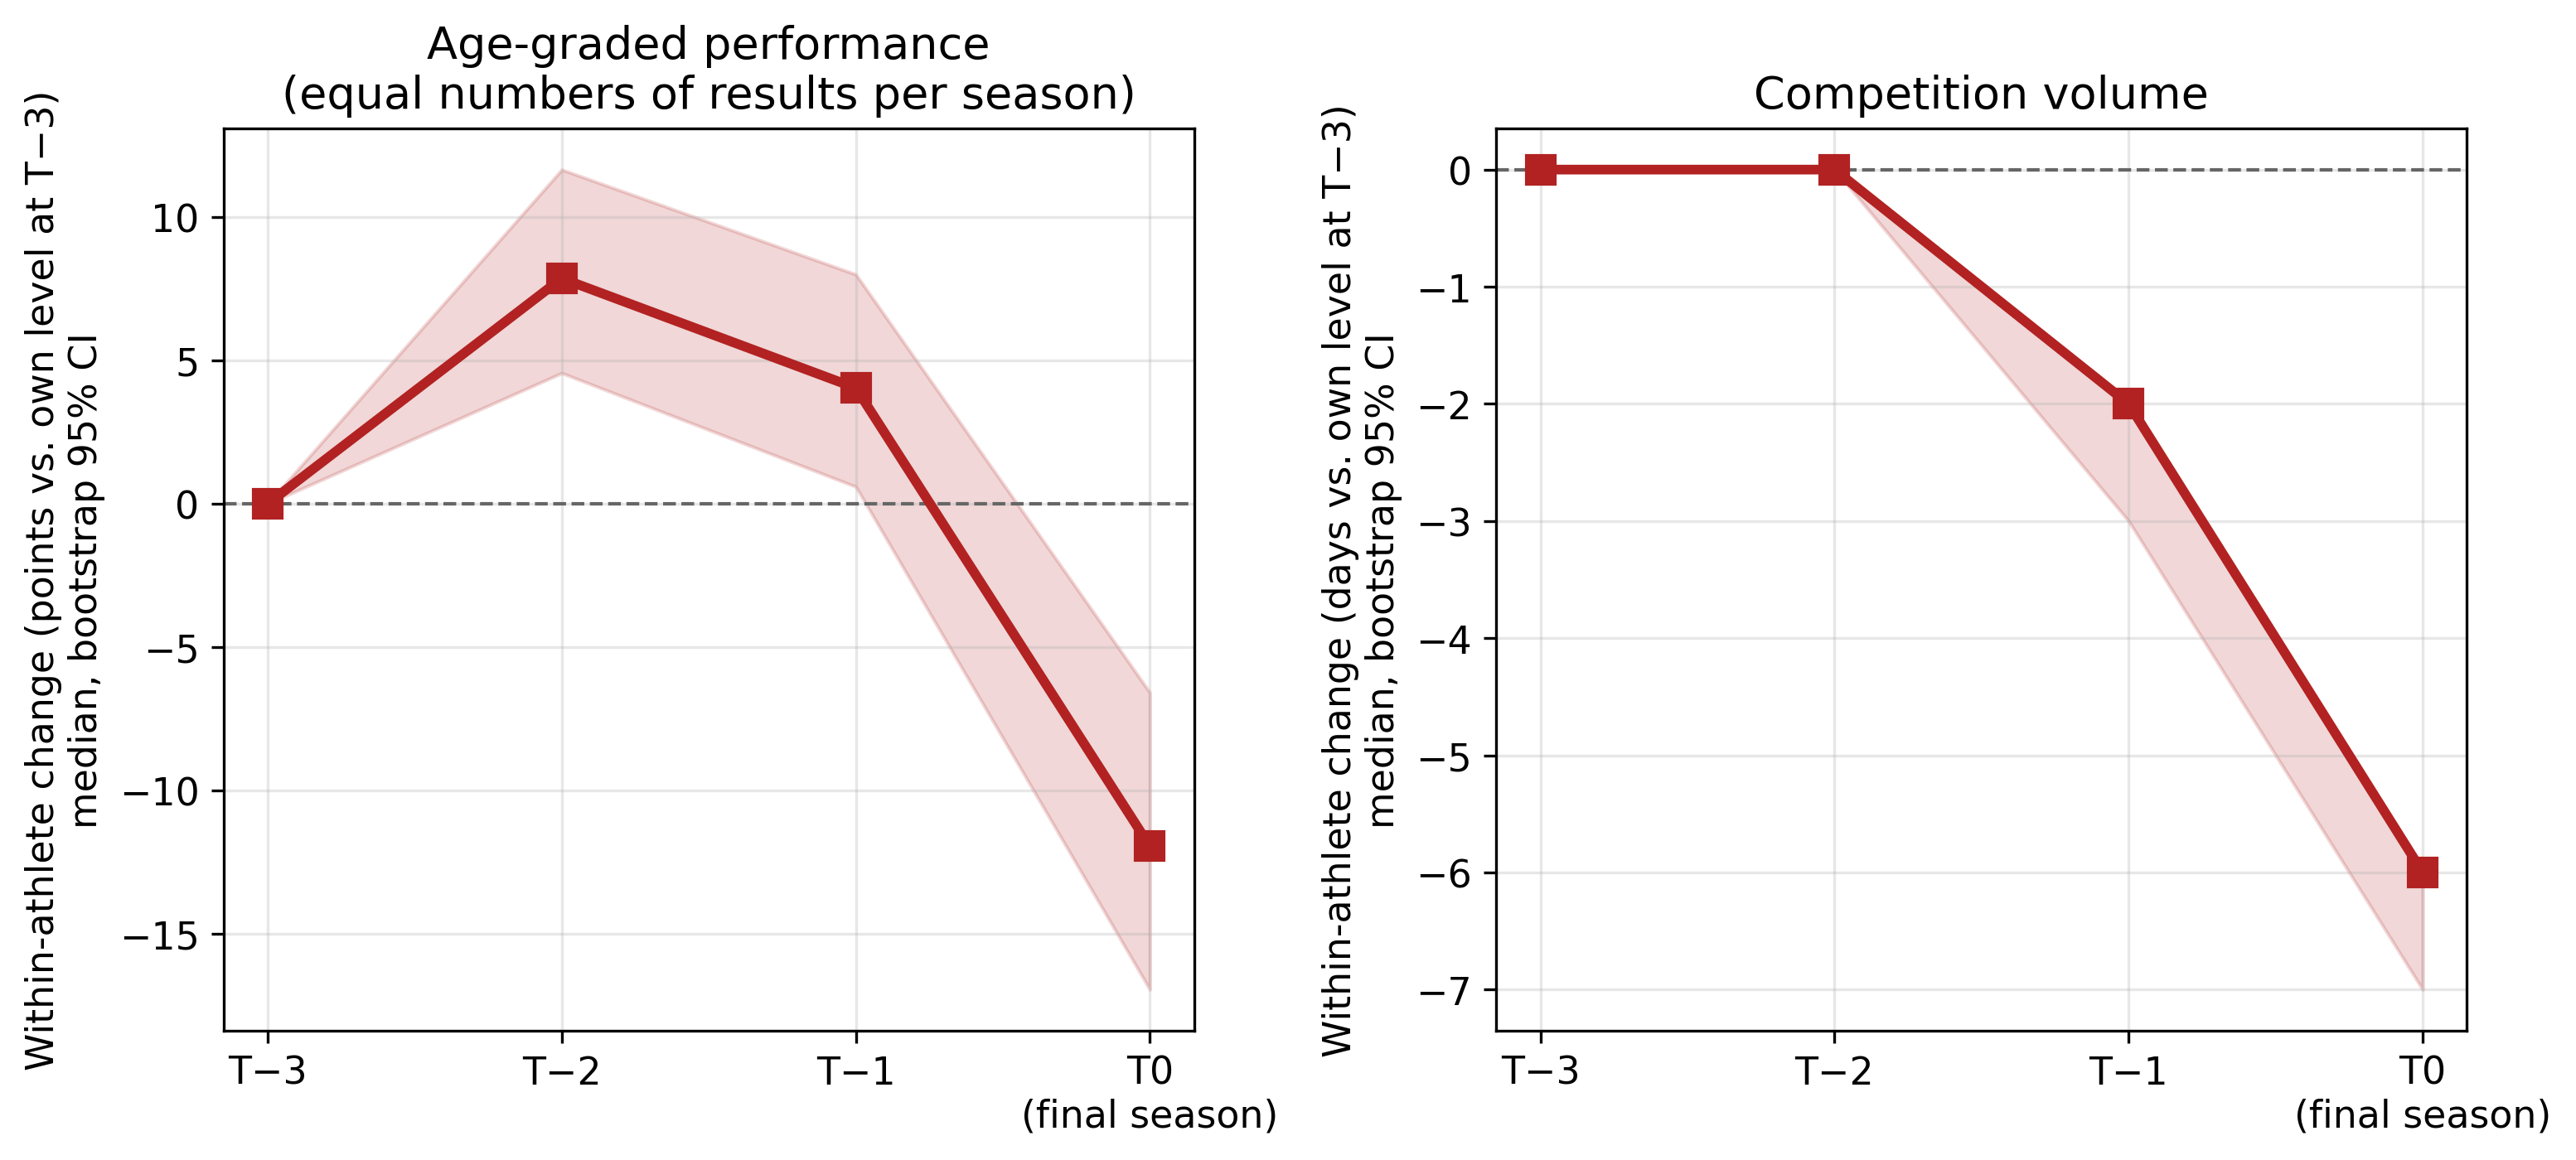
\includegraphics[width=\textwidth]{fig3_exit_aligned.png}
\caption{Within-athlete change over the four last active seasons among dropouts with a final season at ages 16--19 (medians with bootstrap 95\,\% CIs, relative to the athlete's own level three seasons before exit). Left: age-graded performance, compared at equal numbers of results per season (points; n = 1\,116 of the 1\,968 non-censored dropouts with a final season at 16--19, those with scorable main-group results in all four seasons --- a persistent-competitor selection). Right: competition volume (days; n = 1\,523). Abbreviation: CI, confidence interval.}
\label{fig:slide}
\end{figure}

\subsection{Time-to-event and robustness}

In the landmark Cox model among the 2\,001 athletes still competing after age 16, progression was associated with a lower hazard of exit (HR 0.84 per SD, 95\,\% CI 0.79--0.90), alongside level (HR 0.77), later volume (HR 0.73 per SD), null earlier volume given later (HR 1.13), and a higher hazard for women (HR 1.29, 95\,\% CI 1.17--1.42); Kaplan--Meier curves by progression tertile separated from the landmark onward (Figure~\ref{fig:km}). Table S2 in the Supplementary material collects the robustness analyses: the primary OR was stable across exposure definitions (season best 2.09; wind-legal marks 2.17; equal numbers of results in both windows 1.88; event-equated points 1.94; outdoor marks only 1.98; progression in the best event group at 15--16, estimated inclusively on all athletes scorable in that group, with baseline level and result counts from the same group --- n = 3\,990, recovering 318 of the 578 excluded from the primary definition and 15 of the 20 in small cells while 220 primary athletes drop out of it --- 2.53, 95\,\% CI 2.13--3.01; 1.87, 95\,\% CI 1.64--2.12, under the analysis plan's specification, which keeps level and counts from the original main group although the best group differs from it for 31\,\% of the sample), held with spline terms for result counts and volumes (2.15), strengthened when progression was measured from at least two or three results per window (2.39 and 2.53), remained clear among the 2\,001 athletes still competing after age 16, whose final season lies beyond the progression window (1.83, 95\,\% CI 1.55--2.17), held without the COVID-affected cohorts (2.12) with no clear COVID interaction (1.30, CI 0.98--1.74), held across outcome definitions (2.00--2.30; attenuated to 1.55 for the nearer outcome of activity at $\geq$18), replicated almost identically in the two cohort halves (2.20 and 2.24), and was unchanged under club-clustered inference. Regression to the mean does not drive the estimate: with both period levels in the model, the earlier level carried a negative coefficient given the later one (OR 0.75 per 100 points, 95\,\% CI 0.66--0.85), the opposite of what a baseline-measurement artefact would produce. The within-baseline specification check was null (OR 1.03, 95\,\% CI 0.91--1.17), but it has little power against result-count artefacts and is not relied on. The E-value for the primary estimate was 2.36 (2.10 for the CI bound): an unmeasured confounder would need a risk-ratio association of about 2.4 with both a one-SD difference in progression and senior activity to explain the association away.

\begin{figure}[H]
\centering
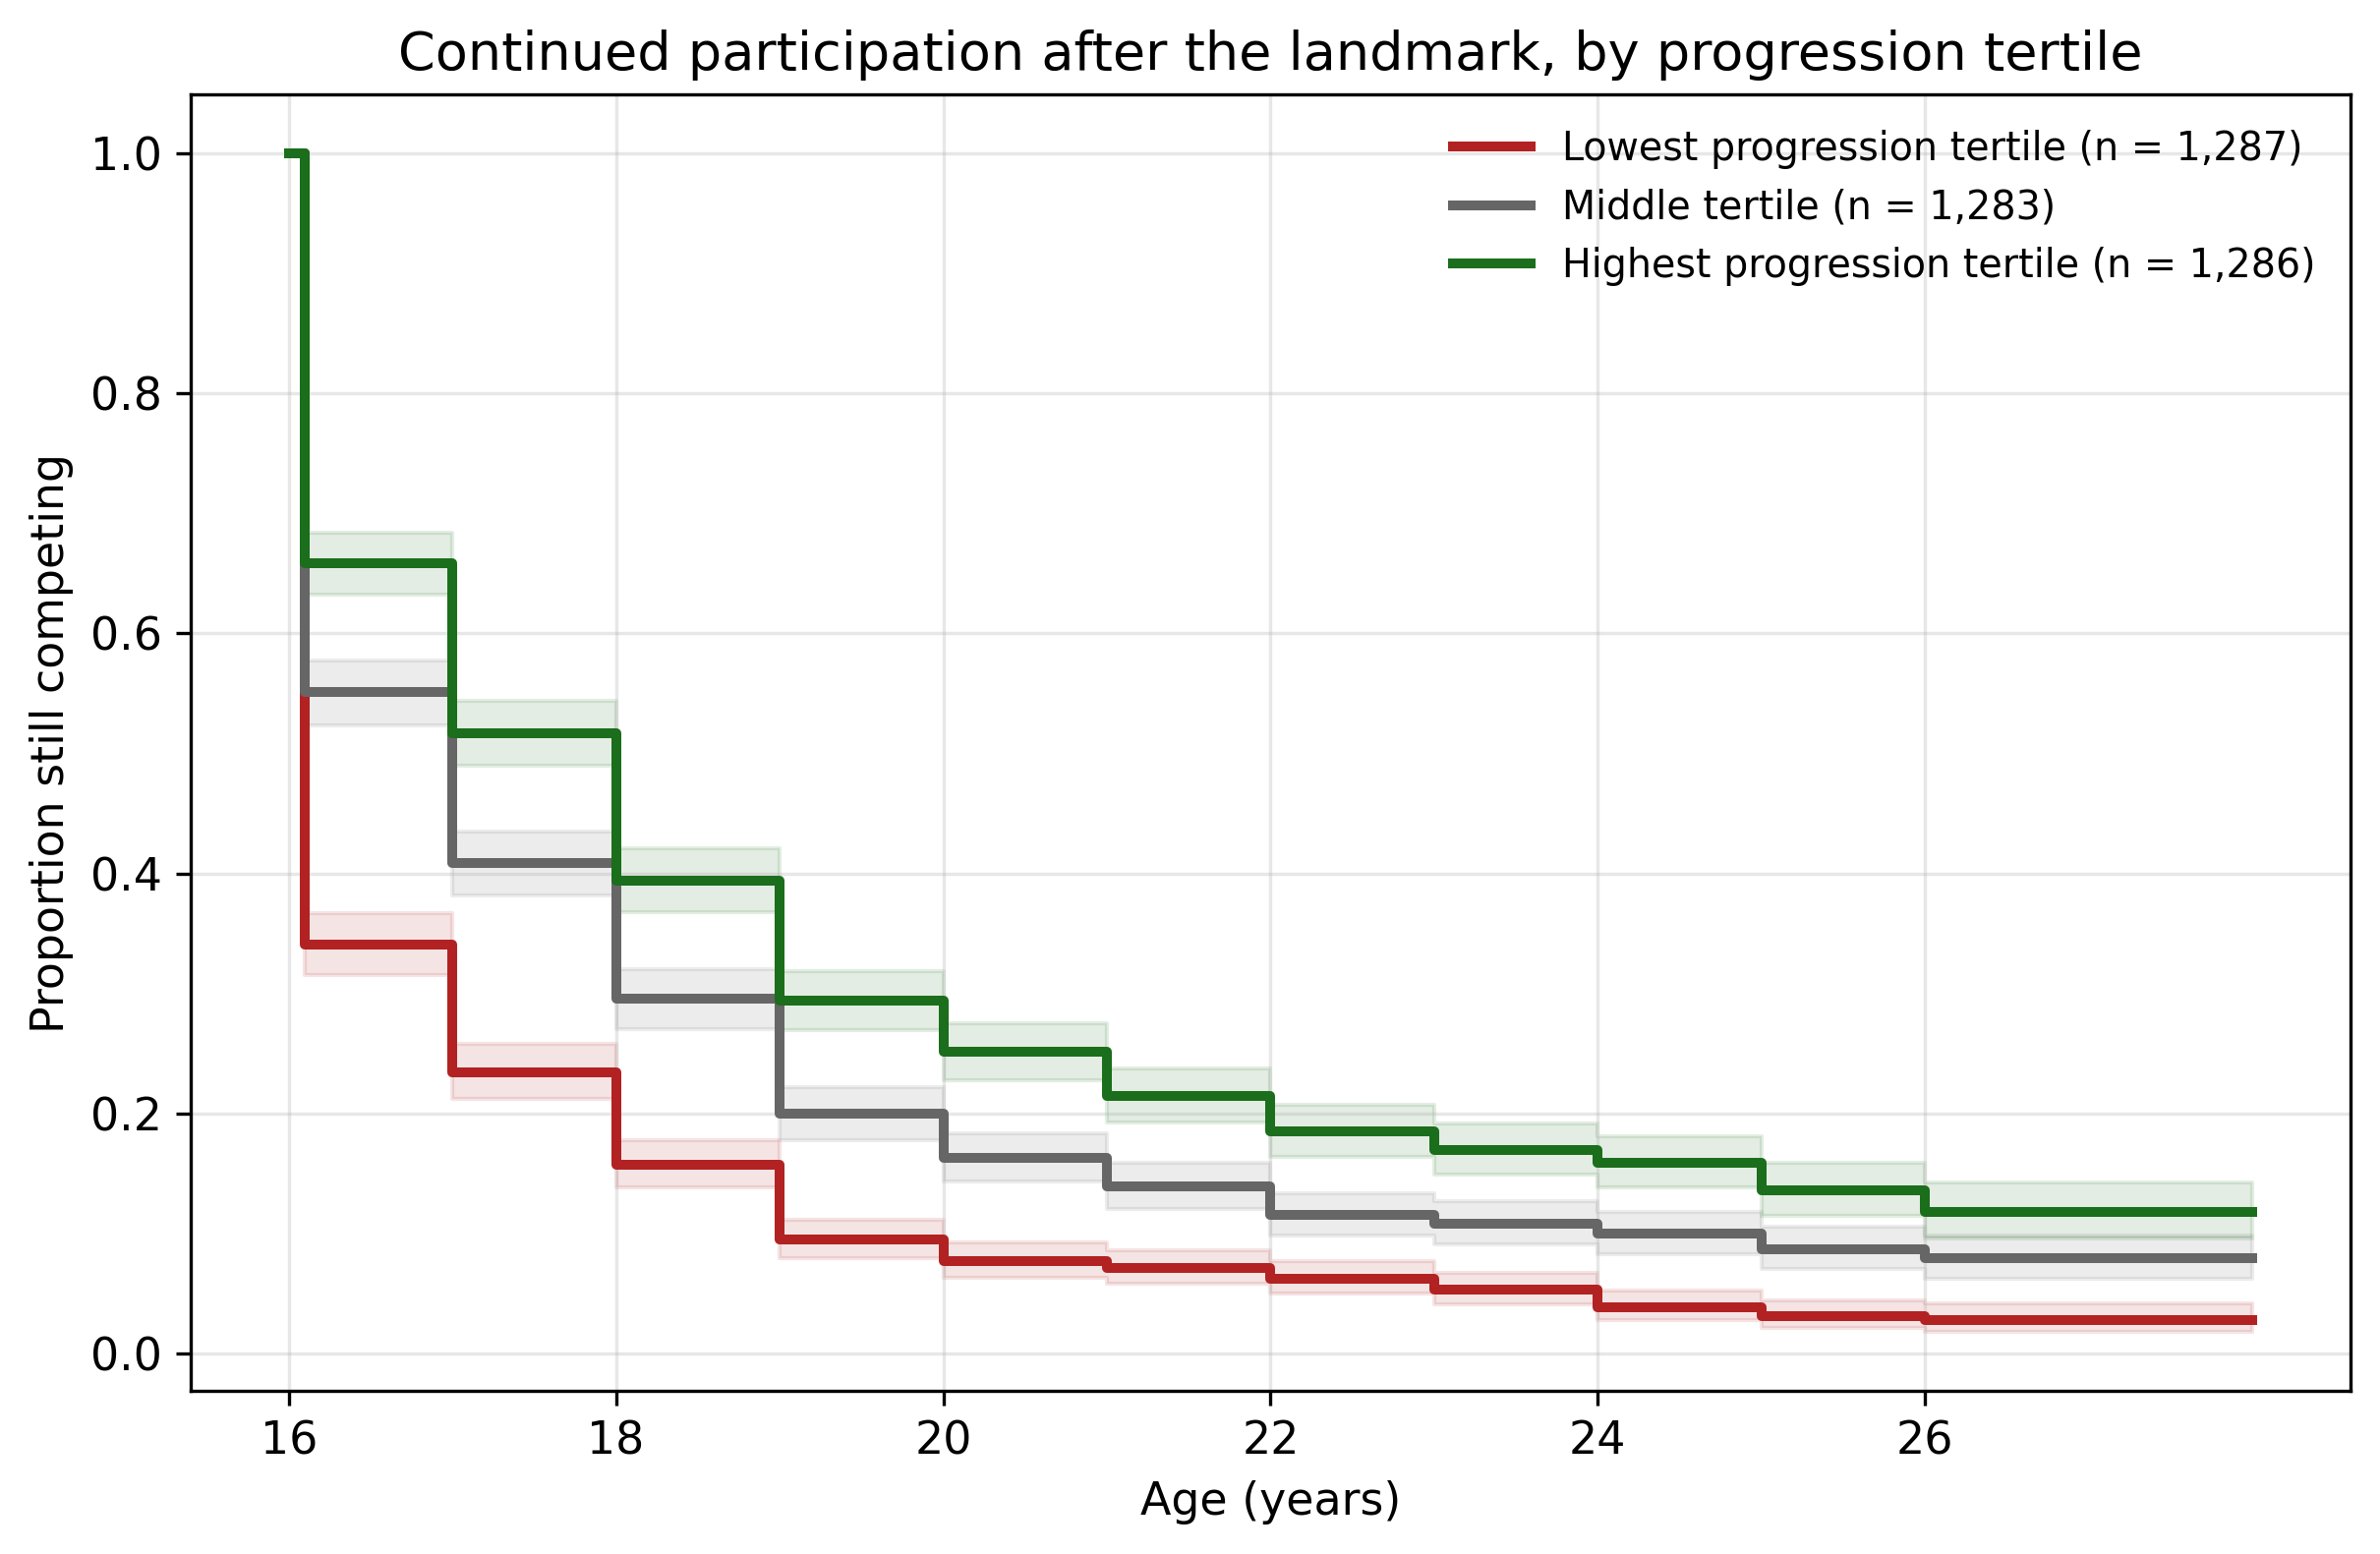
\includegraphics[width=0.85\textwidth]{fig4_km_progression.png}
\caption{Kaplan--Meier curves for continued participation after the landmark, by tertile of progression (tertiles defined in the primary sample), among the athletes still competing after age 16. Time origin is the end of the age-16 season. Athletes active in 2025--2026 are censored; shaded bands are 95\,\% CIs. Abbreviation: CI, confidence interval.}
\label{fig:km}
\end{figure}


\FloatBarrier

% ════════════════════════════════════════════════════════════
\section{Discussion}

\subsection{Principal findings}

In the complete national registry population still competing at ages 15--16, an athlete's own performance progression over early adolescence predicted senior retention with an odds ratio of 2.2 per SD --- of the same order as the baseline competition-volume coefficient reported for the same outcome by \citet{guttormsen2026dropout} (2.04 per SD at ages 13--14), while concurrent volume at 15--16 remains the dominant predictor in the joint model (OR 3.19) --- independently of volume, baseline level, and the number of results, replicated across two birth cohorts, and robust to the pre-specified variations and to comparing the windows at equal numbers of results. Aligned at exit, dropouts with four complete final seasons held their performance level until the final season and fell modestly in it, while their participation was already declining. For most dropouts the progression window contains the final season, so part of the association is the final-season decline itself; among athletes still competing after age 16, whose final season lies beyond the window, the association was smaller but clear (OR 1.83), so low progression also precedes departure. Two pre-specified results bound the finding: the association was no stronger among relatively younger athletes (and a post hoc mediation analysis found only weak evidence for a mediated pathway), and given volume, progression discriminated no better than level.

\subsection{Relation to the earlier studies of the registry}

The result closes the gap the earlier registry studies left open between them. The development study showed that youth top lists turn over because athletes leave and are replaced, without following the leavers \citep{guttormsen2026development}; the cohort study showed that leavers withdraw behaviourally before they exit, without measuring their development \citep{guttormsen2026dropout}. The present study connects the two: the athletes who leave are, disproportionately, the athletes who had progressed least over the preceding windows --- a signal visible in the registry before their departure, alongside their declining participation.

The reparametrisation noted in Methods gives the finding a second, equivalent reading. Because baseline level plus change is the same information as early level plus later level, H1 states that the \emph{later} performance level carries substantial information about retention beyond the earlier one. Current form, not early rank, is what the retention signal tracks. This mirrors, for performance, exactly what \citet{guttormsen2026dropout} found for participation: there too, the later window dominated and the earlier one added nothing given it (both in that study's volume models and in ours); here the earlier performance level even carried a negative coefficient given the later one. The practical reading of both results is the same --- recent behaviour and recent development are what matter, which is also why the incremental \emph{discrimination} from adding progression to a model that already contains later volume is modest (+0.012 AUC). For prediction, participation remains the workhorse; progression adds a description of how the athlete is developing, which participation counts alone do not provide.

\subsection{What this means for the mastery interpretation}

The study was designed as the direct test the relative-age paper called for \citep{guttormsen2026rae}, and the outcome is split in an informative way. What the mastery construct adds beyond a generic ``commitment'' story is the reinforcement claim set out in the Introduction: athletes stay where they can observe their own progress, and the account therefore predicts heterogeneity by access to other reinforcement, rank above all. In this system the signals are concrete: athletes most directly observe times, distances and placings, while age-graded points are printed on Norwegian youth result lists and used for club awards, so the registry's progression measure is an objective correlate of signals athletes actually receive, not a researcher-only abstraction (though it is not perception itself).

The relative-age prediction was tested in its pre-specified moderation form and, post hoc, in a rank-based form, and supported in neither. The birth-quarter moderation was null with the point estimate in the wrong direction, and the more direct rank-based form fared no better: the progression--retention association was present at every baseline level, with no evidence of moderation by level once the reliability of the progression measure was improved by requiring at least three results per window (tertile ORs 2.67, 2.29 and 2.75 among athletes with at least three results per window). The mediated form found little support either: later-born athletes' greater measured progression largely reflected their lower starting level, and birth quarter itself was not associated with senior activity once level and volume were left out. Read against the plan's framing of H2 as the mastery-specific test, the registry evidence favours a general progression--retention link; it shows no reinforcement-deprivation moderation in either tested form, though the intervals leave room for modest moderation, and it offers little support for a mediated mastery pathway. One caveat applies to the null moderation result: relatively younger athletes discouraged early may have left before the landmark, which would bias the test toward the null. In the terms of achievement goal theory, the data also cannot tell whether retained athletes experienced competence through self-referenced improvement or through the rank that improvement also buys; the null moderation shows only that the first source did not visibly compensate for the second where the second was scarcest.

Four processes, none separable in registry data, can produce the general link. Visible progress may sustain motivation (the mastery reading, in its unconditional form). Commitment may run the other way: athletes who have already decided to stay train more and therefore progress more, so that progression partly \emph{measures} commitment rather than causing it. Biological maturation can drive both sides at once: on calendar-calibrated tables a late maturer and a disengaging athlete look alike while the deficit lasts, and maturation timing also shapes exit --- making maturation the leading rival explanation, not an afterthought. And third causes --- injury above all --- can simultaneously halt development and drive exit; injury was the most common stated reason for dropout in the one long-term Norwegian athletics follow-up \citep{enoksen2011} and is invisible in competition records. The same follow-up recorded stagnation in performance among the reasons athletes themselves gave for leaving, which matches the pattern reported here but cannot separate the processes either. The exit-aligned trajectories are equally consistent with all four. What the registry adds is not the mechanism but the observability: whichever process operates, it writes itself into ordinary competition records in the seasons around the athlete's exit.

\subsection{The sex gap persists}\label{sec:sex}

As in the earlier cohort study \citep{guttormsen2026dropout}, women left more often than men with the same volume, level, \emph{and now progression} (OR 0.57; Cox HR 1.29). The gap is not explained by women developing less --- it is conditional on development --- nor by women responding less to their own progress: the progression--retention association was similar in women and men (OR 2.25 in men and 2.21 in women, interaction p = 0.89). Its sources --- which may include competing time demands, environment, and competing priorities and physical factors around puberty documented in the dropout literature \citep{crane2015,fraserthomas2008} --- remain the most consequential unexplained pattern in this registry, and a study of its own.

\subsection{Practical implications}

Norwegian athletics already possesses, in its ordinary results database, both of the early-warning signals the registry studies have now documented: declining participation \citep{guttormsen2026dropout} and, from this study, stagnating or declining age-graded performance among athletes who still compete. For a federation or club, the two signals answer different questions. Falling volume flags \emph{who} is disengaging; falling progression adds information about still-active athletes whose development is stalling. Given the modest incremental discrimination, we would not propose progression-based automated flags; the appropriate use is informal and conversational, and it needs the scale stated. One progression-SD is roughly 114 age-graded points over two seasons; an athlete slipping by that much relative to their own trajectory carries about twice the odds of departure at the group level, and negative progression was nearly twice as common among future dropouts as among retainers when compared at equal numbers of results (45.8 vs.\ 24.3\,\%). But even the median final-season decline (about 12 points, $\approx$0.1 SD) is well inside normal fluctuation for a single athlete --- which is precisely why these are conversation-starters for coaches, not selection or flagging criteria. It also bears saying that leaving one sport in adolescence often reflects competing priorities or a change of activity rather than failure \citep{crane2015,fraserthomas2008}, so the conversation's purpose is understanding, not retention at any cost. The exploratory volume dependence (Figure~\ref{fig:quintile}) suggests the conversation is most valuable while the athlete still competes regularly; once participation has collapsed, progression distinguishes little. Any operational use should respect the governance constraints discussed for behavioural monitoring by \citet{guttormsen2026dropout} (legal basis, designated recipients, opt-out), and none of this evidence supports using progression for talent \emph{selection} --- the development study shows precisely that early rankings understate later development \citep{guttormsen2026development}.

\subsection{Strengths and limitations}

Strengths include national coverage of sanctioned competition from 2011, a landmark design that makes conditioning explicit, an exposure constructed to resist the mechanical maximum-of-$n$ bias, adjusted for result counts and checked at equal numbers of results, internal replication across cohorts, a direct check against regression to the mean, and sensitivity to clustering, COVID-19 exposure, and definitional choices.

The limitations are those of registry research, stated in advance. First, the estimates are associations; no causal effect of progression is claimed, and the four processes above cannot be separated. Second, exit from the athletics registry is not exit from sport: transfer to other sports is invisible, which is why a null H1 would have been uninterpretable --- the asymmetry cuts the other way for the positive finding, since sport transfer would, if anything, generate athletes who leave \emph{while} progressing. Third, injury, training, and biological maturation are unobserved; maturation deserves emphasis, because on calendar-calibrated tables a late maturer whose deficit has not yet closed is indistinguishable from a stagnating athlete, and if late maturers also exit more, the progression--retention association would arise without any motivational mechanism --- the mediated-mastery and maturation readings of the birth-quarter results are observationally equivalent here. Fourth, the age-graded tables are unequally demanding across event groups and across events within a group, so progression partly reflects changes of event; standardisation within sex and event group addresses the group-level differences, and event-equated points (OR 1.94) the within-group ones. Indoor and outdoor marks are pooled (outdoor marks only: OR 1.98). Fifth, the primary definition measures progression within the athlete's original main event group; athletes who changed groups entirely are excluded from the primary analysis, though the switcher-inclusive sensitivity pointed the same way. Sixth, results generalise to athletes still active at 15--16 in an open, club-based, low-cost competition system; absolute rates and thresholds will differ in gate-kept or pay-to-play systems. Finally, the study was not externally preregistered; the analysis plan, hypotheses, estimands, and interpretation rules were committed to version control before any exposure--outcome model was estimated, and the deviations from it are listed in the Supplementary material.

% ════════════════════════════════════════════════════════════
\section{Conclusions}

Among Norwegian youth track-and-field athletes still competing at ages 15--16, within-athlete performance progression predicted senior retention beyond volume and level --- with a conditional odds ratio of the same order as the baseline-volume signal reported previously, though concurrent volume remains the dominant predictor --- while performance itself held until the final season and declined modestly in it. Current form, not early rank, is what the retention signal tracks. The association was general --- similar among early- and late-born athletes, in women and men, and across baseline levels --- while neither the reinforcement-deprivation nor the mediated form of the mastery mechanism found clear support. Competition records thus contain two complementary signals of disengagement: athletes pull back, and they progress less, in the seasons around their exit. What the registry adds is not the mechanism but the observability; understanding why --- commitment, injury, biological maturation, or motivation --- requires data the registry cannot provide, and is the natural next step.

% ── Abbreviations (SMO: list of abbreviations) ──────────────


% ── End matter (PSE) ────────────────────────────────────────

\section*{Data availability}

\noindent The competition records used in this study are publicly accessible via the Norwegian Athletics Federation's online register. The derived analysis dataset cannot be publicly shared because it contains personal data (athlete dates of birth) under the EU General Data Protection Regulation (GDPR). The full analysis code, with the time-stamped analysis plan and the aggregate estimation files, will be deposited in a public repository upon acceptance.

\section*{Supplementary material}

\noindent Table S1 (sample flow), Table S2 (robustness analyses), Section S3 (deviations from the analysis plan) and the completed STROBE checklist accompany the submission.

\section*{Declaration of generative AI and AI-assisted technologies in the manuscript preparation process}

\noindent During the preparation of this work the author used Anthropic Claude to improve language and readability, assist with structuring the text, check analysis code and identify errors. The author has checked the terms of use of the tool. After using this tool, the author reviewed and edited the content as needed and takes full responsibility for the content of the published article.

\printbibliography

\end{document}
